\emph{Konstruktion:} Man zeichnet die beiden Kräfte in einem gewählten Massstab vom selben Punkt aus unter dem Winkel $\alpha = \alKO$ und ergänzt sie zum Kräfteparallelogramm. Die Diagonale ist die resultierende Kraft $\vec F_\text{R}$. Ihre Länge, im Massstab zurückgerechnet, ergibt etwa \FReP{0}{2}.
\begin{center}
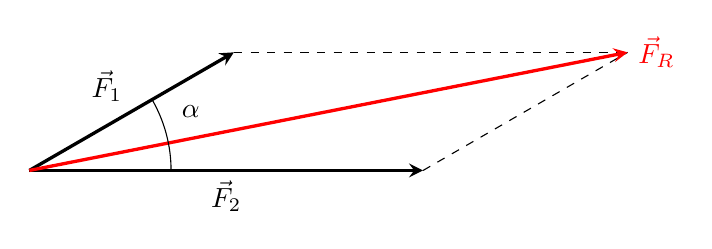
\begin{tikzpicture}[>=stealth]
 \draw[->, very thick] (0,0) -- (5,0);
 \node[below] at (2.5,0) {$\vec F_2$};
 \draw[->, very thick] (0,0) -- (2.598,1.5);
 \node[above left] at (1.3,0.75) {$\vec F_1$};
 \draw[dashed] (5,0) -- (7.598,1.5);
 \draw[dashed] (2.598,1.5) -- (7.598,1.5);
 \draw[->, very thick, red] (0,0) -- (7.598,1.5) node[right] {$\vec F_\text{R}$};
 \draw (1.8,0) arc (0:30:1.8);
 \node at (2.05,0.75) {$\alpha$};
\end{tikzpicture}
\end{center}

\emph{Rechnung:} Im Dreieck aus $\vec F_2$, der verschobenen Kraft $\vec F_1$ und $\vec F_\text{R}$ liegt der Winkel $\SI{180}{\degree}-\alpha$ gegenüber von $F_\text{R}$. Der Kosinussatz mit $\cos(\SI{180}{\degree}-\alpha) = -\cos\alpha$ ergibt
\begin{align}
 F_\text{R} &= \FReF \\
   &= \sqrt{\left(\FEi\right)^2+\left(\FZw\right)^2+2\cdot\FEi\cdot\FZw\cdot\cos\alKO} \\
   &= \FRe \approx \result{\FReP{0}{2}}
\end{align}
